\documentclass[10pt]{beamer}

\usetheme{moloch}

\usepackage{booktabs}
\usepackage[scale=2]{ccicons}

\usepackage{pgfplots}
\usepgfplotslibrary{dateplot}
\usepackage{tikzpeople}
\usepackage{tikz}
\usetikzlibrary{overlay-beamer-styles}
\usetikzlibrary{backgrounds}

\usepackage{fontawesome5}
\usepackage{amsmath}
\usepackage{amssymb}
\newcommand{\kkk}{\mathbf{k}}
\newcommand{\KKK}{\mathbf{K}}
\newcommand{\rrr}{\mathbf{r}}
\newcommand{\iNTT}{$\mathsf{iNTT}$}
\newcommand{\bch}{\mathsf{BCH}}
\newcommand{\intt}{\mathsf{iNTT}}
\newcommand{\leap}{\textsc{Leap}}
\usepackage{xcolor}
\definecolor{mBGcol}{HTML}{fafafa}
\definecolor{colA}{HTML}{990099}
\definecolor{colC}{HTML}{b6b6b6}
\definecolor{colB}{HTML}{00b300}
\definecolor{colD}{HTML}{2eb8b8}
\definecolor{thirdColor}{HTML}{6A5ACD}


\newcommand{\bv}[1]{\mathbf{#1}}
\usepackage[lambda,landau,operators,probability,sets,logic,advantage,complexity,asymptotics,notions,mm,primitives,ff,adversary,advantage]{cryptocode}


\title{ Small Moduli, Big Impact: Toward Communication-Efficient Lattice-Based OPRFs}
\date{1$^{st}$ of December, 2025}
\author{Lena Heimberger}
\institute{Monash University}
\titlegraphic{\vspace{-2em}
\includegraphics[height=1cm]{figures/logo.pdf}\hfill
\includegraphics[height=1cm]{figures/monash.png}}
\pgfplotsset{compat=1.18}

\begin{document}

\maketitle


    % Post-quantum Oblivious Pseudorandom Functions face a major adoption hurdle: their communication overhead is dramatically higher than that of classical elliptic-curve schemes. While lattices offer speed and ease of implementation, traditional constructions like 2-Hash-DH often negate these benefits, forcing complex blinding/unblinding proofs. In our recent paper Leap [1], we challenged the traditional trade-off between communication and computation. Instead, we propose to sacrifice round-optimality to achieve both small computation and communication. This initially seems like a poor compromise, but may be a realistic shift for batched applications and resource-constrained IoT environments.
    % In the talk, I will demonstrate how using a Naor-Reingold PRF (evaluated obliviously) instead of 2-Hash-DH allows us to utilize heuristic Learning With Rounding (LWR) assumptions with very small parameters. Then I'll show some weaknesses, especially in the existing Leap parameter regimes, and how to fix them by reducing the parameters even further, potentially as small as $q=16$ (rounding to $p=2$). This simple, yet powerful construction achieves a communication complexity in the same ballpark as elliptic curves (around 2 KB) and is potentially a lot faster- at a rather new computational model.

\begin{frame}
  \frametitle{Hi!}
  \begin{itemize}
    \item PhD student @Graz University of Technology \\ Supervisor:
      Christian Rechberger\pause
    \item I study lattice-based OPRFs from heuristic assumptions to get
      \alert{efficient} OPRFs. \pause
    \item Recently built an OPRF more efficient than elliptic
      curves!~\cite{EC:HKLMRR25}\pause
    \item Needs more analysis: 
      \begin{itemize}
        \item Lower bounds: How big does the LWR modulus have to be in theory? \pause
        \item Concrete lattice attacks on small-moduli instantiations \pause
        \item underlying PRF: can we find differentials within small-moduli
          PRFs? \\ joint work with
      Sonja Denk (Master student @ TUG)\pause
    \item efficient preprocessing from PQ-OT without KEM\pause
    \item verifiable Naor-Reingold PRFs and consistency proofs 
  \end{itemize}

  \end{itemize}
\end{frame}

 \begin{frame}
   \frametitle{Graz, Austr$_{al}$ia, Republic of }
 
   \begin{figure}
     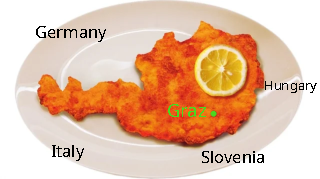
\includegraphics[scale=1.5]{figures/graz.pdf}
     \caption{Schnitzel map from
     \url{https://www.reddit.com/r/mapporncirclejerk/comments/e3x9h4/map\_of\_austria\_but\_its\_actually\_a\_schnitzel/},
     modified by me. }
   \end{figure}
 
 \end{frame}
 
% Brief intro to OPRFs: what they are and why we care
% Key applications: private set intersection, password-authenticated key exchange, privacy-preserving authentication
% Real-world motivation: Why PSI matters for contact discovery, private databases, threat intelligence sharing

\begin{frame}
  \frametitle{Motivation for Oblivious Pseudorandom Functions}
  \begin{itemize}
    \item simple(r) primitive from asymmetric cryptography\pause
    \item gives rise to a number of cool constructions
    \item cheap! \pause...pre-quantum
  \end{itemize}
  \begin{exampleblock}{Pseudorandom Function}
    A pseudorandom function~(PRF) \cite{C:GolGolMic84,GolGolMic86} is a
    deterministic and polynomial time function $F \colon
    \{0,1\}^k\times\{0,1\}^x\rightarrow \{0,1\}^y$ such that
    there is no probabilistic polynomial-time algorithm
    to distinguish any output $y$ from a randomly chosen element from $\{0,1\}^y$.
    \label{def:prf}
  \end{exampleblock}
\end{frame}

\begin{frame}
  \frametitle{Definitions}
  \centering
  \begin{tikzpicture}[every node/.style={minimum width=1.5cm},scale=0.8]

    \node[alice, monitor, shirt=blue!40!black, minimum size=1.5cm, label=Client] (alice)
      {};
    \node[scale=2.67, label=Server, xshift=3.5cm] (server) {{\large{\faServer}}};
    \node[scale=2.67, label=compute, xshift=1.9cm] (hashfunction) {\({y
      \coloneqq F_k(c)}\)};

    \node(Alicetext) [below of=alice,xshift=1cm, yshift=-0.8cm,text
      width=3cm, text=gray]{input \(c \in \mathcal{C}\), gets \(y\)};;
    \node(Servertext) [below of=server, xshift=0.5cm,yshift=-0.5cm,text
      width=3cm,text=gray]{key \(k\in \mathcal{K}\)};;
  \end{tikzpicture}
  \begin{exampleblock}{Oblivious Pseudorandom Function}
    An oblivious pseudorandom function~(OPRF)~\cite{TCC:FIPR05} is a protocol between two parties. One
    party holds the secret key $k$ and the other holds their secret input $x$.
    The OPRF privately realizes the joint computation outputting $F_k(x)$ for a PRF $F$ to the
    party holding $x$, and nothing to the party holding $k$.
    \label{def:oprf}
  \end{exampleblock}

\end{frame}

\begin{frame}{Additional Properties}
  \begin{description}
    \item[Partial Obliviousness] In a POPRF, the client submits a tag $t$ in addition to the
      input $x$ and gets the evaluation $y
      \coloneqq F_k (t, x)$. $t$ contains  additional information,
      e.g. a validity period.\pause
    \item[Threshold] Get a valid evaluation from a $t$-out-of-$n$ servers.\pause
    \item[Verifiability] The client can ensure that a pre-commited server key $k$ was used to compute $y = F_k
      (x)$. \\ VOPRF+POPRF=VPOPRF\pause
    \item[Public Verifiability] means we built a blind signature.
  \end{description}
\end{frame}
  
  \begin{frame}{How would an ideal OPRF look like?}
    %gold standard: 3HashDH OPRF~\cite{EC:TCRSTW22}
    \begin{description}
      \item[Security.] ideally malicious security, i.e. a malicious adversary cannot
        learn anything they shouldn't \pause (doesn't imply detection)\pause
      \item[Round-Optimality.] A \alert{round} is a period where all parties can
        exchange messages simultaneously. \\ \pause A non-interactive protocol (e.g.  NIZK):
        single round, interactive protocol: two rounds \pause
      \item[Communication size.] Elliptic curve OPRFs: 766
        bits of communication. Best lattice-based: tens of kilobytes, in
        a semi-honest setting and with preprocessing.\pause
      \item[Computational complexity.] Generic lattices are fast, and we can speed them up
        further using vector instructions or even GPUs. \\\pause
        Kyber768 takes between a third to half of the
        computational time of ECDH Curve 25519!
    \end{description}
  \end{frame}
  \begin{frame}{Anything else?}
    \begin{description}
      \item[Preprocessing.]  Repeated
        computations? Shift data-independent communication and computation to a
        preprocessing phase.  \pause Fully online protocols: online variant or
        perform the precomputation on the fly.\pause
      \item[Trusted Setup.] In addition to preprocessing, some OPRFs rely on a
        trusted setup.\pause But: trust is a hard problem in itself,
        and sometimes a trusted setup just isn't available (e.g. for
        CSIDH).
    \end{description}
  \end{frame}
 

  \begin{frame}{OPAQUE}
    \hspace{-10em}
    \procedureblock[mode=text]{}{%
      \> \textbf{Client} (pwd)  \> \> \textbf{Server} (k)\\
      \textbf{1. Registration:} \> \(k' = F_{k}(pwd)\) \> \sendmessagerightleft*[16em]{OPRF} \> \\
      \> Sample \((pk, sk)\) \> \sendmessageright*[16em]{pk, ct=Enc_{k'}(sk)} \> Store \((pk, ct)\)\\
      \uncover<2->{
        \textbf{2. Login:} \>\>\sendmessageleft*[16em]{ct} \>\\
        \> \(k' = F_{k}(pwd)\) \>\sendmessagerightleft*[16em]{OPRF} \> \\
        \> \(sk = Dec_{k'}(ct)\) \>\sendmessagerightleft*[16em]{\text{AKE using }sk} \>
      }
      }
      \uncover<3->{
        \hspace*{\fill} \alert{Which properties are important?}
      }
  \end{frame}
  
  \begin{frame}{OPAQUE: Properties}
    \begin{itemize}
      \item doesn't reveal output\pause
      \item server still passively observes the success or failure of an authentication
        attempt\pause
      \item OPRF must be secure against a malicious server\pause
      \item Verifiability?
    \end{itemize}
  \end{frame}
  
  
  \begin{frame}{Private Set Intersection~(PSI)}
    OPRFs are useful for \alert{unbalanced} sets, where one party, typically the
    server in client-server protocols, has a significantly larger set than the other party.
    \begin{figure}
      \centering
      \procedureblock[mode=text]{}{%
        \textbf{Alice} \((x_{1}, \ldots, x_{m})\) \> \> \textbf{Bob} \((y_1,
        \ldots, y_n), k\)\\
        \({\{F_{k}(x_i)\}}_{i \in [m]}\) \> \sendmessagerightleft*[16em]{OPRF
        } \> \\
        \> \sendmessageleft*[16em]{\{z_j = F_k(y_i)\}_{j \in [n]}} \>\\
        }
        \(F_{k}(x_i) = z_{j}\).
        Otherwise \(F_{k}(y_j)\) is pseudorandom.
    \end{figure}\pause
    \hspace*{\fill} \alert{Which properties are important?}
  \end{frame}
  
  \begin{frame}{PSI: Properties}
    \begin{itemize}
      \item per-client keys may cause segmentation \pause
      \item semi-honest server may be realistic: \pause
        \begin{itemize}
          \item regulatory and reputational incentives~\cite{USENIX:KRSSW19}\pause
          \item inherent trust\\ government agencies identifying duplicate entries\pause
          \item anywhere where PSI is applied to limit the risk of data breaches
            \pause
        \end{itemize}
      \item PSI can be a good base case for non-traditional OPRFs
    \end{itemize}
  \end{frame}

\section{Naor-Reingold and Lattices}
\begin{frame}{Naor-Reingold PRF~\cite{NaoRei04}}
  \begin{itemize}
    \item The Naor-Reingold PRF~\cite{NaoRei04} that generically builds a PRF
      from an Abelian group action $*$.\pause
    \item
      To compute the PRF over $m$ input bits, we sample $m+1$ group elements $[g_0,
      g_1, \ldots, g_m]$. \pause
    \item Start with group action with $g_0$.\pause
    \item For every following
      group element, the group action is performed when the $i^{th}$ bit of the input is set. \pause
    \item Automatically hashes to group! \pause
  \end{itemize}
  \begin{example}[Naor-Reingold with seven input bits]
    For example, for $0110111$ we would
    compute the group action $g_0*g_2*g_3*g_5*g_6*g_7$.
  \end{example}\pause
  \alert{Good framework to study group actions!}
\end{frame}

\begin{frame}{Learning with Rounding PRFs}
  \begin{itemize}
    \item \alert{derandomize} Learning with errors \pause
      \begin{itemize}
        \item SIS: $\bv{As}=\bv{x}$
        \item LWE: add noise to get approximate solution $\bv{As}+\bv{e}=\bv{x}$
        \item LWR: round from big modulus $p$ to smaller modulus $q$\\ 
          $\lfloor\bv{As}_q\rceil_p$\pause
      \end{itemize}
    \item NIST PKE/KEM Finalist: Saber~\cite{NISTPQC-R3:SABER20}\pause
    \item Naor-Reingold PRF from LWR: 
  \end{itemize}
  \onslide<1->{
    \begin{align*}
      \mathcal{F}_{\bv{K}}(c_1,
      \cdots,c_m)=S\left(\bv{k}_0 \prod_{i=1}^m \bv{k}_{i}^{c_i}\right)
    \end{align*}
  }


\end{frame}

\begin{frame}{\textsc{Spring} is a lattice-based PRF}
  \begin{itemize}
    \item 2014: \alert{heuristic} LWR PRF with small modulus\pause
    \item two modes: \pause
      \begin{itemize}
        \item \textsc{Spring-BCH} with $q=257$\pause
        \item \textsc{Spring-CRT} with $q=514$\pause
      \end{itemize}
    \item \cite{EC:HKLMRR25} focus in \textsc{Spring-BCH}: rounding bias reduction using extended BCH code
      $[128,64,22]$\pause
  \end{itemize}

  \onslide<3-6>{
    \begin{figure}[H]
      \label{Spring:PRF}
      \vspace{-1em}
      \begin{align*}
        \mathcal{F}_{\bv{K}}(c_1,
        \cdots,c_m)=S\left(\kkk_0 \prod_{i=1}^m \kkk_{i}^{c_i}\right)
      \end{align*}
    \end{figure}
  }

  \onslide<7>{
    \begin{figure}[H]
      \label{Spring:PRF-intt}
      \vspace{-8em}
      \begin{align*}
        \mathcal{F}_{\bv{K}}(c_1,
        \cdots,c_m)=S\left(\intt\left(\kkk_0\odot \prod_{i=1}^m \kkk_{i}^{c_i}\right)\right)
      \end{align*}
    \end{figure}
  }

  \onslide<8>{
    \begin{figure}[H]
      \label{Spring:PRF-intt-lookup}
      \vspace{-8em}
      \begin{align*}
        \mathcal{F}_{\bv{K}}(c_1,
        \cdots,c_m)=S\left(\intt\left(\mathsf{lookup}\left(\kkk_0+
        \sum_{i=1}^m {c_i}\kkk_{i}\right)\right) \right)
      \end{align*}
    \end{figure}
    Multiplication is addition of exponents! \\ 
    \vspace*{-1em}
    \begin{align*}
      g^ag^b= g^{a+b}~\text{for some generator $g$}
    \end{align*}
  }
\end{frame}

\begin{frame}{Why $q=\{257\}$?}
  \begin{itemize}
    \item Choice of modulus from ease of implementation: 
    \item $q=257$
      \begin{itemize}
        \item only use \alert{invertable} polynomials \pause \\ 
        \item Computation mod $q$: use units (nonzero coefficients) \pause \\
          avoid zeroing out 
        \item Fermat's Theorem for prime $q$: 
          \begin{align*}
            g^{q-1}\equiv g^0 \equiv 1 \mod q 
          \end{align*}\pause
        \item use subset-sum of exponents instead of multiplication \pause
        \item Sample in exponent form $\mod q-1= 256$\pause \\ 
          fits in a single byte!
      \end{itemize}
  \end{itemize}
\end{frame}

\begin{frame}{Why $q=\{514\}$?}
  \begin{itemize}
    \item Even modulus $q=514=2*257$\pause
    \item 257-component as on previous slide\pause
    \item 2-component $R_2^*$; 257-style\pause\\ 
      polynomial multiplication $\rightarrow$ coefficient multiplication
      $\rightarrow$ coefficient addition
      \begin{itemize}
        \item polynomial is \alert{invertible} when sum of coefficients is
          odd\pause
        \item Polynomial is represented in \alert{power representation}: $A(x)=x_0+b_1x_1+b_2x_2+...+b_{127}x_{127}, b_i\in \{0,1\}$\pause \\
        \item 2-component is evaluated similar to $257$-component 
      \end{itemize}
  \end{itemize}
\end{frame}

%  \begin{frame}{OPRF-friendly $q$}
%    \begin{itemize}
%      \item some issues with $q=257$ and oblivious evaluation\pause \\
%        \alert{maybe later}\pause
%      \item PRF needs to be fast, OPRF, esp. from lattices, needs to have small
%        communications\pause
%      \item We need some distance between $p$ and $q$, $\approx 3$ bits\pause
%      \item Compose out of $\mod 2$ constructions: $q=16=2*2*2*2$
%    \end{itemize}
%  \end{frame}
% 
%  \section{Almost a symmetric cipher:\\ Spring mod 16}
% 
%  \begin{frame}{Symmetric structure}
%    \vspace*{-2em}
%    \begin{figure}[H]
%      \begin{align*}
%        \mathcal{F}_{\bv{K}}(c_1, \cdots, c_m) = \uncover<4->{\color{colD}}S\left(
%          \uncover<3->{\color{thirdColor}} \intt\left(
%            \uncover<2->{\color{colA}} \mathsf{lookup}\left(
%              \uncover<1->{\color{colB} \kkk_0 + \sum_{i=1}^m {c_i}\kkk_{i}}
%            \right)
%          \right)
%        \right)
%      \end{align*}
%    \end{figure}\pause
%    \begin{itemize}
%      \item {\color{colB} Key addition }\pause
%      \item {\color{colA}Substitution }\pause
%      \item {\color{thirdColor}Permutation }\pause
%      \item {\color{colD}Truncation}\pause
%      \item Optional round function through CTR mode for longer outputs
%    \end{itemize}
%  \end{frame}
% 
%  \begin{frame}{Efficient Subset-Products}
%    Let's zoom into the computation $\mod 2$
%    \vspace*{-2em}
%    \begin{figure}[H]
%      \begin{align*}
%        \mathcal{F}_{\bv{K}}(c_1, \cdots, c_m) = S\left(
%          \intt\left(
%            \mathsf{lookup}\left(
%              \uncover<1->{{\color{colB} \kkk_0 + \sum_{i=1}^m {c_i}\kkk_{i}}}
%            \right)
%          \right)
%        \right)
%      \end{align*}
%    \end{figure}
%    \begin{itemize}
%      \item to make it efficient, we change the representation twice: 
%        \begin{enumerate}
%          \item power basis (final result): $x^j$ \pause\\
%            Multiplication is expensive $O(n^2)$
% 
%          \item radix basis (intermediate representation): $(1+x)^j$\pause\\
%            Freshman's dream: $(1+x)^j\equiv 1+x^j \mod 2$
% 
%        \end{enumerate}
% 
%      \item Shift-and-XOR through exponent representation \pause
%      \item abstract idea: $g^ag^b\equiv g^{a+b}$
%    \end{itemize}
%  \end{frame}
% 
% 
% \begin{frame}{Efficient Subset-Sum in $R_2^*$ via the exponent representation}
%   \begin{itemize}
%     \item We need a generator $g=3 \mod 257$
%        \item Break $R_2^*$ into cyclic components: 
%          $C_2^{n/4} \times C_4^{n/8} \times C_8^{n/16} \times \ldots
%          \times  C_n$\pause
%        \item \alert{exponent representation}: $j$ represents $1+(1+x)^j$\pause
%        \item Each $C_i$ component is cycic, so it generates a part of the group\pause
%        \item Every element can be rewritten as
%          $g_{0,0}^{e_0}g_{1,1}^{e_1}g_{1,3}^{e_2}\ldots g_{\log_n,0}^{e_63}$\\ 
%          $e$ are small integer exponents. \pause
%        \item Multiplication of cyclic components is addition: 
%          \begin{itemize}
%            \item 32 1-bit expontents: XOR
%            \item add 2-bit to 7-bit exponents and only keep LSB\pause
%            \item parallelizable!
%          \end{itemize}
%      \end{itemize}
%  \end{frame}
%  \begin{frame}{Substitution}
%    \vspace*{-2em}
%    \begin{figure}[H]
%      \begin{align*}
%        \mathcal{F}_{\bv{K}}(c_1, \cdots, c_m) = S\left(
%          \intt\left(
%            {\color{colA} \mathsf{lookup}}\left(
%              \kkk_0 + \sum_{i=1}^m {c_i}\kkk_{i}
%            \right)
%          \right)
%        \right)
%      \end{align*}
%    \end{figure}
%    \begin{itemize}
%      \item given $a$, compute $g^a\mod q$
%      \item alternative $\mod 2$: Exponent to radix representation
%    \begin{itemize}
%     \item Multiplying $A(X)$ by $(1+x)^j$ means a leftshift by $j$.\pause
%        \item 
%          Multiplying by $1+(1+x)^j$
%          \begin{align*}
%            A(x)\oplus (A(x)\ll j)
%          \end{align*}
% %         The nice thing is we can just XOR the 1-bit exponents, and add the other
% %         exponents and then apply a mask. this is constant-time! and... now
%        \item multiply out components using shift-and-xor\pause
%          Final form: $(x+1)^j$
%    \end{itemize}
% 
%    \end{itemize}
%  \end{frame}
% 
%  \begin{frame}{Permutation (Radix to power form)}
%    \vspace*{-2em}
%    \begin{figure}[H]
%      \begin{align*}
%        \mathcal{F}_{\bv{K}}(c_1, \cdots, c_m) = S\left(
%          {\color{thirdColor}
%        \intt}\left(
%            \mathsf{lookup}\left(
%               \kkk_0 + \sum_{i=1}^m {c_i}\kkk_{i}
%            \right)
%          \right)
%        \right)
%      \end{align*}
%    \end{figure}
%        $A(x)=c_0*1+c_1*(1+x)+c_2*(1+x)^2+...+c_{127}*(1+x)^{127} $\pause \\
%    \begin{itemize}
%      \item Cooley-Tukey Radix 2 evluation: 
%        \begin{itemize}
%          \item instead of $g$ we have the bases $\{1, (1+x), (1+x)^2, \ldots, (1+x)^{127}\}$
%          \item $c_i \in \{0,1\}$\pause
%           \item Same polynomial, different representation: 
%             \begin{align}
%               A(x)(1+x)^j=\sum_i^{127}c_i(1+x)^{i+j}
%             \end{align}
%          \item \alert{Multiplying $A(X)$ by $(1+x)^j$ means a leftshift by $j$ }
%          \item recursive operation: if 
% 
%            exploit that $(1+x)^{j}\equiv 1+x^{j}$
% 
%            %So, in the radix basis, we just expand the terms. 
% 
%            % Let's say we have $b = [b_0,b_1,b_2,b_3]$ in radix basis.
% 
%            % We can recursively expand the basis basis
% 
%          \item can also be done with shifts and masks 
%            %       (n=8, xor positions that differ by
%            %       four first, then two, then one) 
%            % This represents:
% 
%        \end{itemize}
% 
%    \end{itemize}
%  \end{frame}
% 
%  \begin{frame}[fragile]
%    \frametitle{Truncation}
%    \vspace*{-2em}
%     \begin{figure}[H]
%       \begin{align*}
%         \mathcal{F}_{\bv{K}}(c_1, \cdots, c_m) = {\color{colD}S}\left(
%           \intt\left(
%             \mathsf{lookup}\left(
%              \kkk_0 + \sum_{i=1}^m {c_i}\kkk_{i}
%             \right)
%           \right)
%         \right)
%       \end{align*}
%     \end{figure}
%     \begin{itemize}
%       \item Rounding function
%     \[
%           \lfloor a\rceil_p = \begin{cases} 
%             1 & \frac{q}{4}\leq a\geq \frac{3q}{4}\\
%             0 & \text{otherwise}
%           \end{cases}
%         \]\pause
%       \item alternatives possible, e.g. MSB rounding\pause
%       \item combine composition of results\pause
%       \item e.g. $\mod 16$: four computations $\mod 2$\pause
%       \item design is less clear
%     \end{itemize}
%  \end{frame}

 \section{Oblivious Evaluation}

 \begin{frame}{A little help from MPC friends}
   \centering
   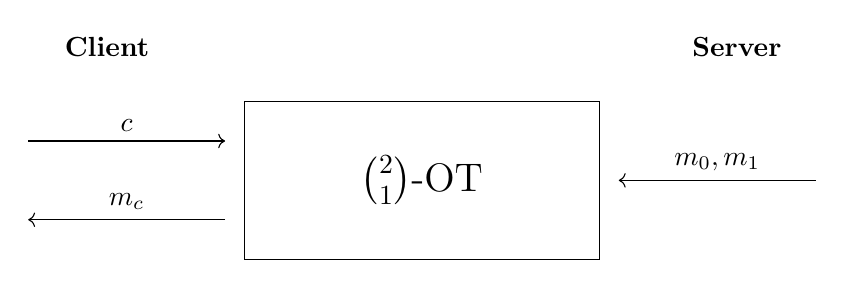
\begin{tikzpicture}
     \node[text centered] at (-4, 1.7) {\textbf{Client}};
     \node[text centered] at (4, 1.7) {\textbf{Server}};

     \node[draw, text centered, minimum width= 4.5cm, minimum height=2cm] at
       (0,0){\Large{$2\choose 1$-OT}};
     \draw[->](5, 0) -- (2.5, 0)node[midway,above]{$m_0, m_1$};

     \draw[->] (-5, 0.5)  -- (-2.5, 0.5) node[midway,above]{$c$};
     \draw[->] (-2.5, -0.5) -- (-5, -0.5) node[midway,above]{$m_{c}$};
   \end{tikzpicture}
   \pause

   \vspace{1em}
   \alert{Extend} with symmetric operations!
 \end{frame}

 \begin{frame}{A little help from MPC friends (cont.)}
   \centering
   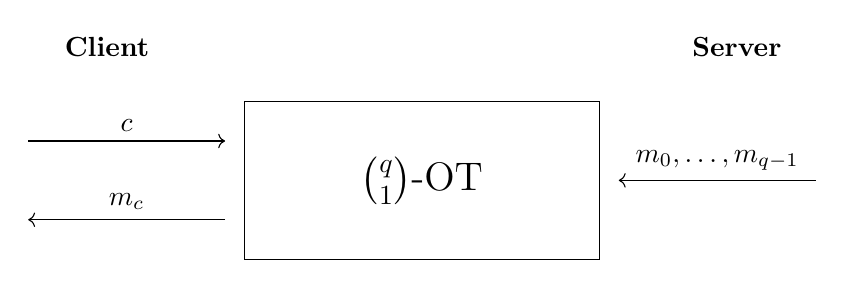
\begin{tikzpicture}
     \node[text centered] at (-4, 1.7) {\textbf{Client}};
     \node[text centered] at (4, 1.7) {\textbf{Server}};

     \node[draw, text centered, minimum width= 4.5cm, minimum height=2cm] at
       (0,0){\Large{$q\choose 1$-OT}};
     \draw[->](5, 0) -- (2.5, 0)node[midway,above]{$m_0, \ldots, m_{q-1}$};

     \draw[->] (-5, 0.5)  -- (-2.5, 0.5) node[midway,above]{$c$};
     \draw[->] (-2.5, -0.5) -- (-5, -0.5) node[midway,above]{$m_{c}$};
   \end{tikzpicture}
   \pause

   \vspace{1em}
   Generic construction from \alert{${\log q}$ $2\choose 1$-OTs} !
 \end{frame}

 \begin{frame}{A little help from MPC friends (cont.)}
   \centering
   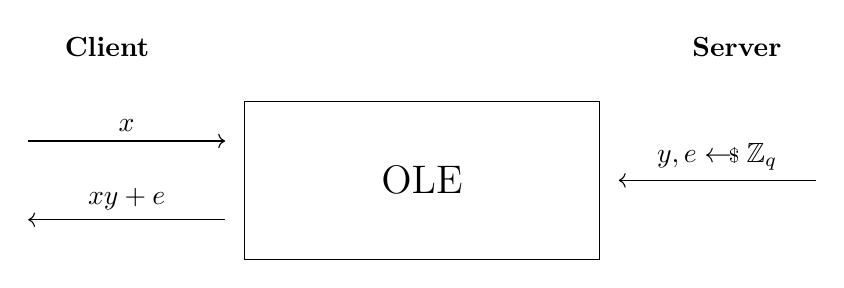
\begin{tikzpicture}
     \node[text centered] at (-4, 1.7) {\textbf{Client}};
     \node[text centered] at (4, 1.7) {\textbf{Server}};
     \node[draw, text centered, minimum width= 4.5cm, minimum height=2cm] at
       (0,0){\Large{OLE}};
     \draw[->](5, 0) -- (2.5, 0)node[midway,above]{$y, e\sample \ZZ_q$};

     \draw[->] (-5, 0.5)  -- (-2.5, 0.5) node[midway,above]{$x$};
     \draw[->] (-2.5, -0.5) -- (-5, -0.5) node[midway,above]{$xy+e$};
   \end{tikzpicture}
   \pause

   \vspace{1em}
   Generic construction from \alert{${\log q}$ $2\choose 1$-OTs} !
 \end{frame}
 %
 %   %%%%%%%%%%%%%%%%%%%%%%%%%%%%%%%%%%%%%%%%%%%%%%%%%%%%%%%%%%%%%%%%%%
 %
 \begin{frame}{Leap}
   \begin{itemize}
     \item Leap~\cite{EC:HKLMRR25}: Naor-Reingold LWR OPRF! \pause
     \item very fast online: can shift almost everything to the preprocessing phase\pause
     \item online phase takes less than a millisecond\pause
     \item \alert{symmetric-style} evaluation\pause
     \item optimized for PSI
   \end{itemize}
 \end{frame}

 \begin{frame}{An OPRF from \textsc{Spring}}
   \begin{columns}
     \hspace*{0.1em}
     \vspace*{-3em}
     \begin{column}{.48\textwidth}
       \begin{figure}
         \begin{align*}
           \only<1-2>{
             \color{colC}S\left(\intt\left(\mathsf{lookup}\left(\color{black}\kkk_0+
             \sum_{i=1}^m {c_i}\kkk_{i}\color{colC}\right)\right)\right)
           }
           \only<3-5>{
             \color{colC}S\left(\intt\left(\color{black}\mathsf{lookup}\left(\kkk_0+
             \sum_{i=1}^m {c_i}\kkk_{i}\right)\color{colC}\right)\right)
           }
           \only<6-7>{
             \color{colC}S\left(\color{black}\intt\left(\mathsf{lookup}\left(\kkk_0+
             \sum_{i=1}^m {c_i}\kkk_{i}\right)\right)\color{colC}\right)
           }
           \only<8->{\color{black}
             S\left(\intt\left(\mathsf{lookup}\left(\kkk_0+ \sum_{i=1}^m {c_i}\kkk_{i}\right)\right)\right)
           }
         \end{align*}
       \end{figure}
     \end{column}
     \begin{column}{.67\textwidth}
       \centering
       \vspace*{-3em}
       \resizebox{\textwidth}{!}{
         \begin{tikzpicture}[background rectangle/.style={fill=mBGcol}, show
           background rectangle]
           % Label for Client on the left and Server on the right
           \uncover<1->{
             \node[text centered] at (-4, 2) {\textbf{Client}};
             \node[text centered] at (-4, 1.4) {$\bv{c}=[c_1, \ldots, c_m] \in
               \{0,1\}^m$};
             \node[text centered] at (4, 2) {\textbf{Server}};
             \node[text centered] at (4, 1.4) {$\bv{K}=[\kkk_0, \kkk_1, \ldots, \kkk_m] \in
               \{0,1\}^m$};

             \node[draw, text centered, minimum width= 4.5cm, minimum height=2cm] at
               (0,0){\Large{$2\choose 1$-OT}};
             \draw[->](5, 0) -- (2.5, 0)node[midway,above]{$\bv{r}_i, \bv{r}_i+\kkk_i$};

             \draw[->] (-5, 0.5)  -- (-2.5, 0.5) node[midway,above]{$c_i$};
             \draw[->] (-2.5, -0.5) -- (-5, -0.5) node[midway,above]{$\bv{r}_i+\kkk_i{c_i}$};

           }
           \uncover<2->{
             \draw[line width=0.1 mm] (-5.5,-1.1) -- (5.5,-1.1);
             \node[ text centered, minimum width= 4.5cm, minimum height=1cm] at
               (0,-1.5){$\sum_{i=1}^\kappa \bv{r_i}+c_i \bv{k_i}$\qquad  \qquad\qquad\qquad
               $\kkk_0-(\sum_{i=1}^\kappa \bv{r}_i)$};
           }
           \uncover<3->{
             \node[ text centered, minimum width= 4.5cm, minimum height=1cm] at
               (0,-1.8){\faRecycle};
             \draw[line width=0.2 mm] (-5.5,-2.8) -- (5.5,-2.8);
             \node[ text centered, minimum width= 4.5cm, minimum height=1cm] at
               (0,-2.3){$\bv{b}\leftarrow\prod_{i=1}^\kappa \bv{r_i}\bv{k_i}^{c_i}$\qquad  \qquad\qquad\qquad
               $\bv{a}\leftarrow\kkk_0(\prod_{i=1}^\kappa \bv{r}_i)^{-1}$};
           }
           \uncover<4->{

             \node[draw, text centered, minimum width= 4.5cm, minimum height=2cm] at
               (0,-4){\Large{OLE}};
             \draw[->](-5, -3.6) -- (-2.5, -3.6) node[midway,above]{$b_i$};
             \draw[<-](-5, -4.5) -- (-2.5, -4.5)node[midway,above]{$y_i=a_ib_i+e_i$};
             \draw[<-] (2.5, -4)  -- (5, -4) node[midway,above]{$a_i,
                 e_i \sample
               \ZZ_q$};

             \draw[line width=0.1 mm] (-5.5,-5.1) -- (5.5,-5.1);
           }
           \uncover<5->{
             \node[ text centered, minimum width= 4.5cm, minimum height=1cm] at
               (-0.5,-5.5){$\bv{y}\leftarrow\sum_{i=0}^{n-1} (a_i\cdot b_i + e_i) X^i$\qquad \qquad  \qquad\quad
               $\bv{e}\leftarrow\sum_{i=0}^{n-1} e_i X^i$};
           }
           \uncover<6->{
             \node[ text centered, minimum width= 4.5cm, minimum height=1cm] at
               (0,-6){$\intt$};
           }
           \uncover<7->{
             \node[ text centered, minimum width= 4.5cm, minimum height=1cm,
               visible on=<9->] at
               (0.1,-6.5){\qquad\qquad\qquad\qquad\qquad\qquad\qquad\qquad
               $\bv{d}\sample\{0,1\}^n$};
             \draw[line width=0.2 mm] (-5.5,-7) -- (5.5,-7);
           }
           \uncover<8->{
             \node[draw, text centered, minimum width= 4.5cm, minimum height=2cm] at
               (0,-8.5){\Large{$q\choose 1$-OT}};

             \draw[->](-5, -8) -- (-2.5, -8) node[midway,above]{$y_i$};
             \draw[<-, visible on=<8>](-5, -9) -- (-2.5, -9) node[midway,above]{$\lfloor
               y_i-e_i\rceil_p$};
             \draw[<-, visible on=<9->](-5, -9) -- (-2.5, -9) node[midway,above]{$\lfloor
               y_i-e_i\rceil_p\oplus d_i$};
             \draw[->, visible on=<8>](5, -8.5) -- (2.5, -8.5) node[midway,above]{$\lfloor
               (q_i-e_i)\rceil_p $} ;
             \draw[->, visible on=<9->](5, -8.5) -- (2.5, -8.5) node[midway,above]{$\lfloor
                 (q_i-e_i)\rceil_p\oplus d_i
               $} ;
             \node [text centered] at (4, -9){$ \forall q_i\in \ZZ_q$};
           }
           \uncover<9->{
             \draw[<-, visible on=<9->](-4, -10.25) -- (4, -10.25)
               node[midway,above]{$\mathsf{BCH(\bv{d})}$};
           }
         \end{tikzpicture}

       }
     \end{column}
   \end{columns}
 \end{frame}
 

    \begin{frame}{I am very proud of it}
      \begin{itemize}
        \item[\faCheck] proof in the semi-honest model\pause
        \item two problems make it hard to claim
          malicious security
      \end{itemize}
    \end{frame}
  
    \begin{frame}{Server Attack}
      \begin{itemize}
        \item generic attack on Naor-Reingold OPRFs \pause
        \item only works when the server can
          reason about the OPRF output \pause
        \item either because it is revealed later or because the
          protocol gives information (e.g. whether or not an authentication attempt
          succeeds.)  \pause
      \end{itemize}
  
      \begin{example}[Generic Attack on Naor-Reingold OPRFs]
        Instead of honestly inputting $\kkk_i+\bv{r}_i$ into the $2\choose 1$-OT, a
        malicious server may input some $\Delta_i+\bv{r_i}$ for some $\Delta_i \neq
        \kkk_i$. When the client result is revealed, the server can learn whether or not the
        $i^{th}$ bit is set.
        %  For example, if the authentication
        %  succeeds even though the server inputted $\bv{\Delta}_i$, the server can
        %  conclude that the $i^{th}$ bit of the client is not set. If the authentication
        %  attempt fails, the bit may be set. This is less reliable as the client may have
        %  just mistyped the password, but over multiple runs (e.g. by faulting the other
        %  message) the server can be more sure.
      \end{example}\pause
      Solution? \alert{Verifiable}
      variant of this OPRF. \pause But
      Naor-Reingold keys are rather large which makes the verification less
      efficient. 
    \end{frame}
  
    \begin{frame}{Client Attack}
      \begin{itemize}
        \item Leak public key coefficients by faulting the rounding step of
          the OPRF. \pause
        \item The key observation is that the rounding result is \alert{deterministic
          and constant for fixed inputs}. \pause
        \item Add an offset $\Delta$ to the coefficient and leak the exact point where the rounding
          result flips from zero to one or vice versa. \pause
        \item
          The attack is mitigated by enforcing \alert{consistency} between the OLE output
          and the rounding input so the client cannot compute the offset anymore.
      \end{itemize}
    \end{frame}

    \begin{frame}{Observation on the modulus}
      \begin{itemize}
        \item The BCH attack exploits the rounding bias. \pause
        \item The CRT attack exploits the linearety. \pause
        \item ... combine both to mitigate attack? \pause
        \item We suggested this! \pause \\ Still leak key \alert{offset}, but
          cannot determine actual coefficient \pause
        \item Probability of $\frac{1}{2}^n$ of guessing the correct key! \pause
        \item Cool, but hacky: we leak a lot about the key. The original goal
          was designing lattice PRFs without ZK. 
      \end{itemize}
    \end{frame}
    % 
    \begin{frame}{Let's work it out in the remix}
      \begin{itemize}
        \item Leak everything but the MSB? \pause \alert{Reduce modulus!}\pause
        \item Lattice estimator times out a lot, but $q=16$ seems secure.\pause
          \\ Reduce communication by half!\pause
        \item Would support that the exponential modulus for LWR PRFs is a proof
          artifact! \pause
        \item Lattice attacks? 
      \end{itemize}
    \end{frame}

    \begin{frame}{Conclusion}
      \begin{itemize}
        \item Leap has a proof in the semi-honest model\pause \\
          Some problems to make it malicious secure. \pause
        \item Parameter choice may be sub-optimal.\pause
        \item What is the concrete best attack on tiny moduli? \pause
        \item How to prove malicious security with that much leakage and
          interaction? UC does not work (blind computation).  
      \end{itemize}
    \end{frame}

    \begin{frame}{Acknowledgements}
      \begin{itemize}
        \item Thank you, Sonja, Hannah, Sebastian, Reinhard, Shibam, Markus and Christian
for your helpful comments on an earlier version of this lecture!
        \item       This work is partially funded by the Digital Europe Program under grant
agreement number 101091642 ("QCI-CAT"). 
      \end{itemize}
    \end{frame}
\maketitle
    \begin{frame}[allowframebreaks]
      \frametitle{References}

      \bibliography{bilbio,cryptobib/crypto,cryptobib/abbrev3}
      \bibliographystyle{alpha}

    \end{frame}
    \end{document}
